\chapter{Evaluation}

\section{Measures of Success}

The success of the project can be measured by comparing the project results with objectives. We will also review the design choices in constructing the tool. The review will highlight the practical outcomes from using argumentation to explain scheduling.
\linespace
Arguably, the most important outcome of this project is that the tool is functionality correct. This means the tool is required to explain schedules for feasibility, efficiency and satisfaction with respect to user decisions.
\linespace
One objective is to implement an accessible tool. To measure accessibility, we can refer to the tractability complexity from explanations. The length of explanations either in the number of words or characters may be correlated with understandability. In addition, we conduct a survey targeted towards potential users. Because the understandability of explanations are difficult to measure, we will use open-ended questions. To carefully evaluate explanations, one would need to refer to cognitive science, which is beyond the scope of this project. We will have two groups, one group without access to the tool, another group with access. By using these metrics, we can measure the accessibility of our tool. Moreover, we can measure performance to reflect responsiveness and scalability of the tool. This may be achieved by using profiling utilities to measure performance metrics such as execution time and memory consumption. 

\section{Theoretical Results}

We summarise our complexity results from Chapter \ref{implementation}.

\begin{figure}[H]
	\begin{tabular}{lccc}
		\hline
		Algorithm & Computational & Memory & Tractability\\
		\hline
		\textsc{Construct-Feasibility} & $\mathcal{O}(m^2n^2)$ & $\mathcal{O}(m^2n^2)$ &\\
		\textsc{Construct-Efficiency} & $\mathcal{O}(m^2n^2)$ & $\mathcal{O}(m^2n^2)$ &\\
		\textsc{Construct-Satisfaction} & $\mathcal{O}(m^2n)$ & $\mathcal{O}(m^2n^2)$ &\\
		\textsc{Compute-Unattacked} & $\mathcal{O}(m^2n^2)$ & $\mathcal{O}(mn)$ &\\
		\textsc{Compute-Partial-Conflicts} & $\mathcal{O}(mn)$ & $\mathcal{O}(mn)$ &\\
		\textsc{Explain-Stability} & $\mathcal{O}(m^2n^2)$ & $\mathcal{O}(m^2n^2)$ &\\
		\textsc{Explain-Feasibility} & $\mathcal{O}(mn^2)$ & $\mathcal{O}(mn)$ & $\mathcal{O}(mn)$\\
		\textsc{Explain-Efficiency} & $\mathcal{O}(mn^2\log(mn^2))$ & $\mathcal{O}(mn^2)$ & $\mathcal{O}(mn^2)$\\
		\textsc{Explain-Satisfaction} & $\mathcal{O}(mn)$ & $\mathcal{O}(mn)$ & $\mathcal{O}(mn)$\\
		\textsc{Full-Precomputation-Explain} & $\mathcal{O}(m^2n^2\log(mn^2))$ & $\mathcal{O}(m^2n^2)$ & $\mathcal{O}(mn^2)$\\
		\textsc{Partial-Precomputation-Explain} & $\mathcal{O}(m^2n^2\log(mn^2))$ & $\mathcal{O}(mn^2)$ & $\mathcal{O}(mn^2)$\\
		\hline
	\end{tabular}
	\caption{Computational, memory and tractability complexity of algorithms using argumentation}
\end{figure}

Using an naive explanation approach only improves the computational complexity of verifying the feasibility property, from $\mathcal{O}(m^2n^2)$ to $\mathcal{O}(mn)$.

\section{Practical Results} 

The tool's functionality is demonstrated in the user documentation guide in Appendix \ref{userguide}. We will compare different implementation methods and see how fit for purpose our tool is through a survey.

\subsection{Comparison of Explanation Generation Methods}

We will compare two algorithmic approaches to AAF construction with and the naive approach without argumentation. The algorithms are implemented, then profiled for elapsed time and maximum allocated memory. The time and memory are measured with the Python's \texttt{cProfile} and \texttt{memory-profiler} modules respectively. The tool was executed on Department of Computing's virtual machines, with the specification of dual-core CPU at 2GHz with 2GiB RAM.
\linespace
Time comparison:
\begin{itemize}
	\item Elapsed time measurements are noisy.
	\item For less than 100 jobs, all approaches have approximately equal timings.
	\item From profiling, the tool takes 0.4 seconds on average to startup.
	\item Partial precomputation is 3\% faster than full precomputation on average, excluding startup time.
	\item Naive is 18\% faster than partial precomputation on average, excluding startup time.
	\item Both graphs hints at quadratic complexity.
\end{itemize}

Memory comparison:
\begin{itemize}
	\item For less than 40 jobs, all approaches have approximately equal memory usage.
	\item From profiling, the tool uses 52MiB on average to startup.
	\item For a large number of jobs, partial-precomputation is 7 times more efficient than full precomputation excluding startup memory.
	\item Naive and partial-precomputation have less than 1\% memory usage difference.
	\item Both graphs hints at quadratic complexity.
\end{itemize}

\newpage

\begin{figure}[H]
	\centering
	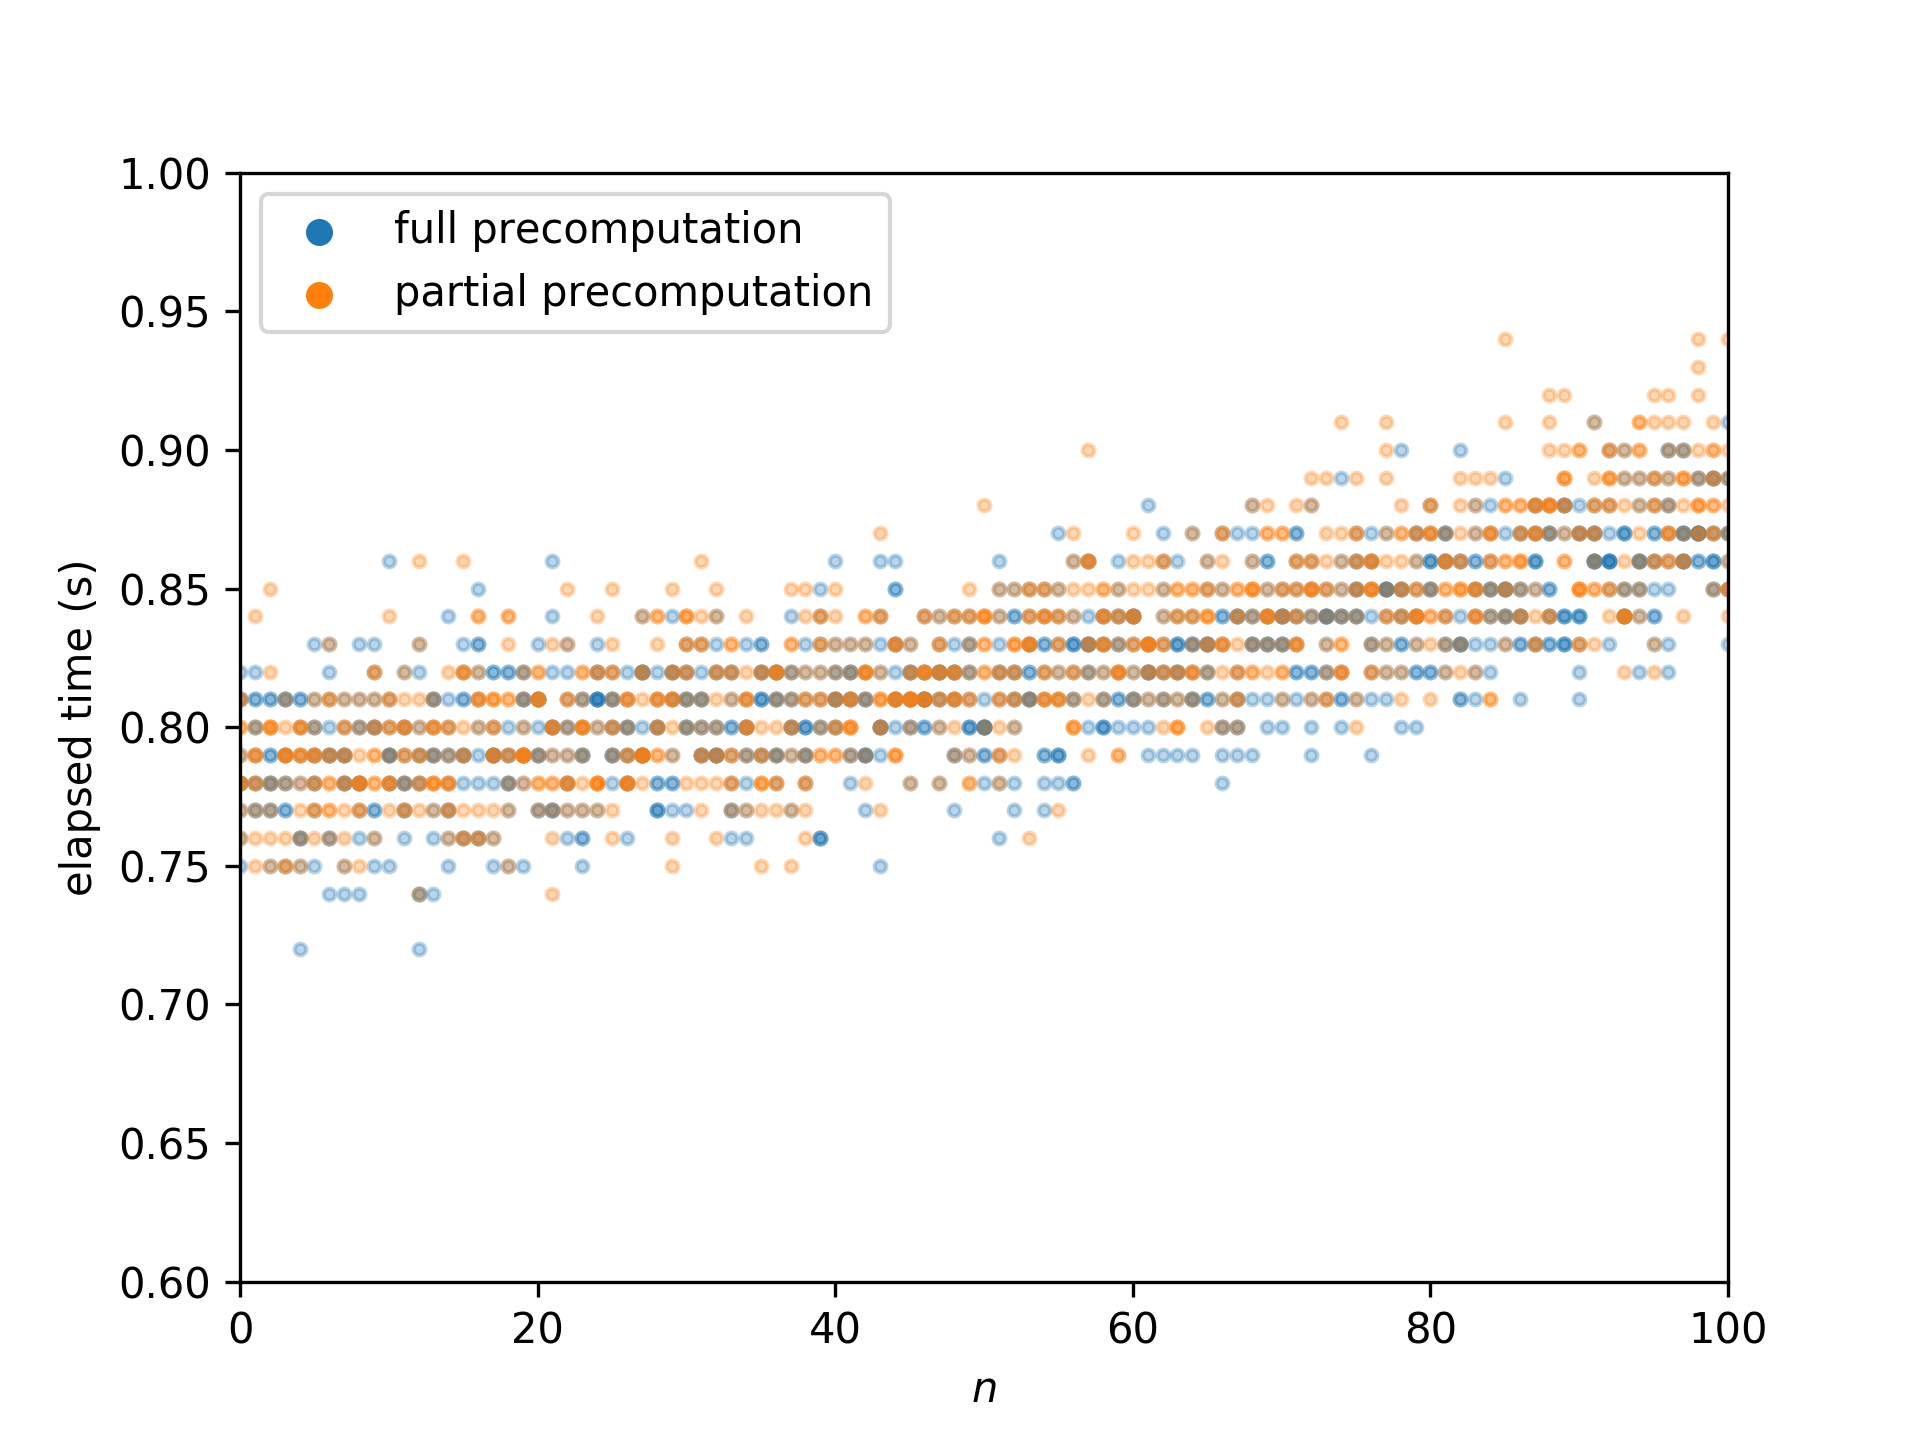
\includegraphics[scale=0.7]{figures/precomputation_cpu_small}
	\caption{Elapsed time comparison where $m=10$ and $0\leq n\leq 100$ with 1000 samples.}
\end{figure}

\begin{figure}[H]
	\centering
	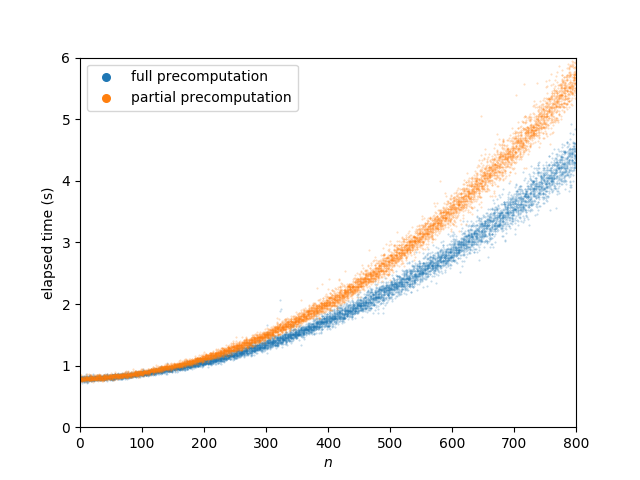
\includegraphics[scale=0.7]{figures/precomputation_cpu_big}
	\caption{Elapsed time comparison where $m=10$ and $0\leq n\leq 800$ with 8000 samples.}
\end{figure}

\begin{figure}[H]
	\centering
	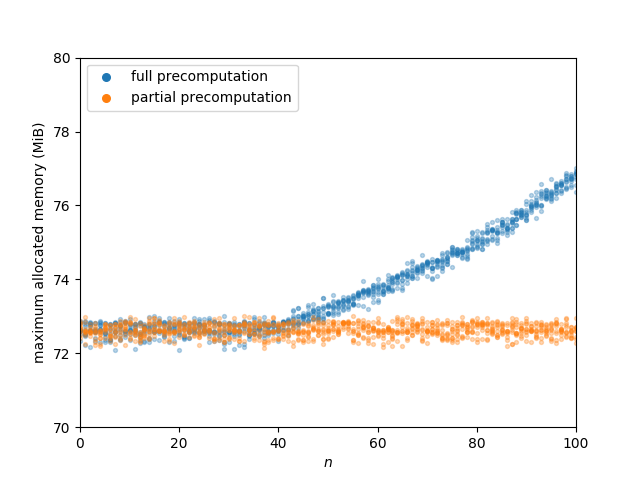
\includegraphics[scale=0.7]{figures/precomputation_memory_small}
	\caption{Maximum allocated memory comparison where $m=10$ and $0\leq n\leq 100$ with 1000 samples.}
\end{figure}

\begin{figure}[H]
	\centering
	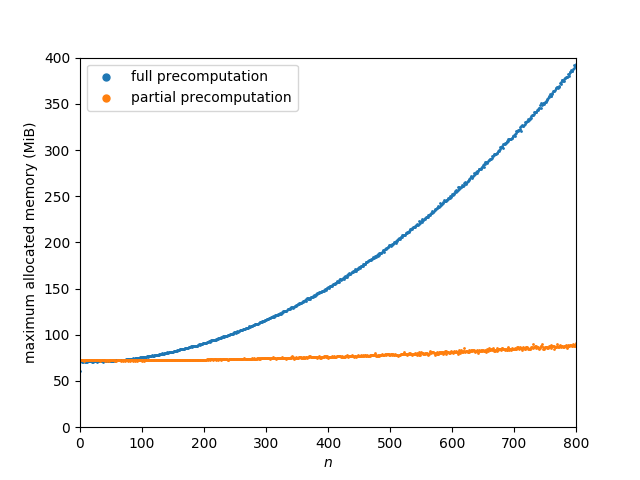
\includegraphics[scale=0.7]{figures/precomputation_memory_big}
	\caption{Maximum allocated memory comparison where $m=10$ and $0\leq n\leq 800$ with 8000 samples.}
\end{figure}

\subsection{Survey Responses}

...

\subsection{Feedback}

During development of the tool, I asked my colleagues and friends for advice about the usability of my tool.

\begin{itemize}
	\item In early versions of the tool, the GUI did not arrange textboxes and buttons into groups such as problem, schedule and explanation. Instead, all buttons and their functionality were exposed as an menu. This was confusing to new users because it was not evident which textboxes were input or output.
	\item The paper \cite{aes} represented machine job pair assignments as a pairs of integer indices. The tool internally uses indices to compute explanations, however exposing both machines and job as integer indices was confusing. Therefore, jobs are now represented alphabetically.
	\item The tool uses regular expressions to validate user input. This was too strict, and users often forgot to input well-formatted white-space. To solve this, the tool automatically corrects missing or surplus white-space.
\end{itemize}